\documentclass[]{article}
\usepackage{lmodern}
\usepackage{amssymb,amsmath}
\usepackage{ifxetex,ifluatex}
\usepackage{fixltx2e} % provides \textsubscript
\ifnum 0\ifxetex 1\fi\ifluatex 1\fi=0 % if pdftex
  \usepackage[T1]{fontenc}
  \usepackage[utf8]{inputenc}
\else % if luatex or xelatex
  \ifxetex
    \usepackage{mathspec}
    \usepackage{xltxtra,xunicode}
  \else
    \usepackage{fontspec}
  \fi
  \defaultfontfeatures{Mapping=tex-text,Scale=MatchLowercase}
  \newcommand{\euro}{€}
\fi
% use upquote if available, for straight quotes in verbatim environments
\IfFileExists{upquote.sty}{\usepackage{upquote}}{}
% use microtype if available
\IfFileExists{microtype.sty}{\usepackage{microtype}}{}
\usepackage[margin=1in]{geometry}
\usepackage{graphicx}
\makeatletter
\def\maxwidth{\ifdim\Gin@nat@width>\linewidth\linewidth\else\Gin@nat@width\fi}
\def\maxheight{\ifdim\Gin@nat@height>\textheight\textheight\else\Gin@nat@height\fi}
\makeatother
% Scale images if necessary, so that they will not overflow the page
% margins by default, and it is still possible to overwrite the defaults
% using explicit options in \includegraphics[width, height, ...]{}
\setkeys{Gin}{width=\maxwidth,height=\maxheight,keepaspectratio}
\ifxetex
  \usepackage[setpagesize=false, % page size defined by xetex
              unicode=false, % unicode breaks when used with xetex
              xetex]{hyperref}
\else
  \usepackage[unicode=true]{hyperref}
\fi
\hypersetup{breaklinks=true,
            bookmarks=true,
            pdfauthor={Justin Le},
            pdftitle={A Brief Primer on Classical and Quantum Mechanics for Numerical Techniques},
            colorlinks=true,
            citecolor=blue,
            urlcolor=blue,
            linkcolor=magenta,
            pdfborder={0 0 0}}
\urlstyle{same}  % don't use monospace font for urls
% Make links footnotes instead of hotlinks:
\renewcommand{\href}[2]{#2\footnote{\url{#1}}}
\setlength{\parindent}{0pt}
\setlength{\parskip}{6pt plus 2pt minus 1pt}
\setlength{\emergencystretch}{3em}  % prevent overfull lines
\setcounter{secnumdepth}{0}

\title{A Brief Primer on Classical and Quantum Mechanics for Numerical Techniques}
\author{Justin Le}
\date{November 29, 2013}

\begin{document}
\maketitle

\emph{Originally posted on
\textbf{\href{http://home.jle0.com:4111/entry/a-brief-primer-on-classical-and-quantum-mechanics.html}{in
Code}}.}

Okay! In this series we will be going over many subjects in both physics and computational
techniques, including the Lagrangian formulation of classical mechanics, basic principles of quantum
mechanics, the Path Integral formatulion of quantum mechanics, the Metropolis-Hastings Monte Carlo
method, dealing with entropy and randomness in a pure language, and general principles in numerical
computation! Fun stuff, right?

The end product will be a tool for deriving the ground state probability distribution of arbitrary
quantum systems, which is somewhat of a big deal in any field that runs into quantum effects (which
is basically every modern field). But the real goal will be to hopefully impart some insight that
can be applied to broarder and more abstract applications. I am confident that these techniques can
be applied to many problems in computation to great results.

I'm going to assume little to no knowledge in Physics and a somewhat intermediate working knowledge
of programming. We're going to be working in both my favorite imperative language and my favorite
functional language.

In this first post I'm just going to go over the basics of the physics before we dive into the
simulation. Here we go!

\section{Classical Mechanics}\label{classical-mechanics}

\subsection{Newtonian Mechanics}\label{newtonian-mechanics}

Mechanics has always been a field in physics that has held a special place in my heart. It is most
likely the field most people are first exposed to in a physics course. To me, there really is no
more fundamental and pure form of physics. I mean\ldots{}it's the study of how things move under
forces. How can you get any deeper to the heart of physics than that?

When most people think of mechanics, they think of \(F = m a\), inertia, and that every reaction has
an equal and opposite re-action. These are Newton's ``Laws of Motion'' and they provide what can be
referred to as a ``state-updating function'': Given a state of the world at time \(t_0\), Newton's
laws can be used to ``generate'' the state of the world at time \(t_0 + \Delta t\).

This sounds pretty useful, but it wasn't long before physicists began wishing they had other tools
with which to study the mechanics of certain systems. Newton's equations worked very well for the
cases that made it famous, but were surprisingly unuseful, impractical, or clumsy in many others.
And when we talk about relativity, where things like \(\Delta t\) can't even be trivially defined,
it is almost completely useless without complicated modifications.

So it was almost exactly one hundred years after Newton's laws that two people named
\href{http://en.wikipedia.org/wiki/Joseph-Louis_Lagrange}{Lagrange} and
\href{http://en.wikipedia.org/wiki/Leonhard_Euler}{Euler} (who is the ``e'' in \(e\)) followed a
wild hunch that ended up paying off.

\subsection{Lagrangian Mechanics}\label{lagrangian-mechanics}

To understand Lagrangian Mechanics, we must abandon our idea of ``force'' as the fundamental
phenomenon. Instead of forces, we deal with ``potential fields''.

You can imagine potential fields as a roller coaster track, or as a landscape of rolling grassy
hills. The height of a track or a landscape at that point corresponds to the value of the potential
at that point. Potential fields work like this: Every object ``wants'' to go \emph{downwards} in a
potential field --- it will want to go in the direction (backwards/forwards for the roller coaster,
north/south/east/west for the hilly landscape) that will take it downwards. We don't care why, or
how --- it just ``wants'' to. And the steeper the downwardness, the greater the compulsion.

We call this potential field \(U(\vec{r})\), which means ``\(U\) at the point \(\vec{r}\)''.
(\(\vec{r}\) denotes a point in space)

Relating this to \(F = m a\), the force on the object is now equal to the steepness of the potential
field at the point where the object is, and in the direction that would allow the object to go
downwards in potential. Objects always wish to minimize their potential, and do so as fast as they
can. In mathematical terminology, we say that \(F(\vec{r}) = - \vec{\nabla} U(\vec{r})\).

\begin{figure}[htbp]
\centering
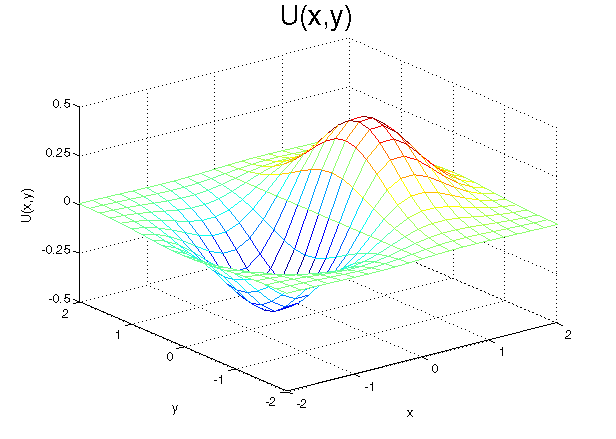
\includegraphics{/img/entries/path-integral-intro/potential3d.png}
\caption{An example of a 2D potential \(U(\vec{r})\).}
\end{figure}

\begin{figure}[htbp]
\centering
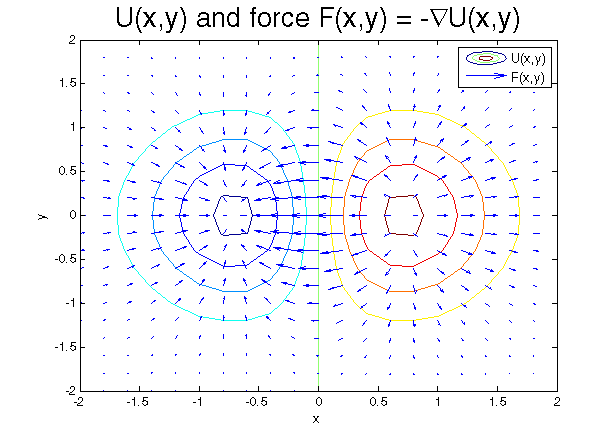
\includegraphics{/img/entries/path-integral-intro/gradient.png}
\caption{Top-down view of the potential in the previous figure, overlayed with arrows indicating the
direction and magnitude of \(F(\vec{r})\).}
\end{figure}

Now, for Lagrangian Mechanics:

Let's say I tell you an object's location at time \(t_0\), and its location later at time \(t_1\),
and the potential energy field. What path did that object take to get from point A to point B?

A pretty open question, right? You don't really have that much information to go off of. You just
know point A and point B. It could have taken any path, for all we know! If we only knew
\(F = m a\), not only would we be at a complete loss at how to even start, but we wouldn't even know
if there was only one or even a hundred valid paths a particle could have taken.

The solution to this problem is actually rather unexpected. Consider every single path/curve from
point A to point B. Every single one. Now, assign each path a number known as the \textbf{Action}:

\begin{enumerate}
\def\labelenumi{\arabic{enumi}.}
\tightlist
\item
  For every point, add up the ``Kinetic Energy'' at that point, which, for classical mechanics, is
  the square of the object's speed multiplied by \(\frac{1}{2} m\).
\item
  For every point, add up \(U(\vec{r})\) at that point.
\item
  Subtract (2) from (1).
\end{enumerate}

Think about every possible path. Calculate the action for each one. The path that the object takes
is \emph{the path with the lowest action}

It's almost as if the object ``does the math'' in its head: ``I'm going to go from here to
there\ldots{}let me calculate which path I can take has the lowest action. Okay, got it!''

Lagrangian Mechanics provides for us a way to find out just what path an object must have taken to
get from point A to point B.

As it turns out, looking at things this way opens up entire worlds of understanding. For example,
just from this, we find that \emph{total energy is conserved} over time for a closed system (trust
me on this; the calculus is slightly tricky). We also have a formulation that works fine under
Special Relativity in all frames of reference with almost no tweaks. And yes, if you actually do
find the path of lowest action, the path will somehow magically always follow the state-updating
equations \(F = m a\). It's just now we have a much more insighftul and meaningful way to look at
the universe:

Paths \textbf{always attempt to minimize their action}.

Okay. We don't have that much time to spend on this, or its philosophical implications, so we're
going to move on now to Quantum Mechanics.

\section{Quantum Mechanics}\label{quantum-mechanics}

\subsection{Schrödinger Formulation}\label{schruxf6dinger-formulation}

If there was one thing that ``everyone'' knew about quantum mechanics, it would either be
\href{http://en.wikipedia.org/wiki/Schr\%C3\%B6dinger's_cat}{Scrödinger's Cat} or the fact that
objects are no longer ``for sure'' anywhere. They are only \emph{probably} somewhere.

How can we then analyze the behavior of \emph{anything}? If everything is just a probability, and
nothing is certain, we can't really use the same ``state-updating functions'' that we used to rely
on, because the positions and velocities of the objects in question don't even have well-defined
values.

Physicists' first solutions involved creating a new ``state'' that did not involve particles at all.
This ``state'' described the state of the universe, but not in terms of particles and positions and
velocities. It is a new \emph{abstract} state. Then, they invented the equivalent of an \(F = m a\)
for this abstract state --- an equation that, for every abstract state at time \(t_0\), gives you
the abstract state at time \(t_0 + \Delta t\).

This approach is useful\ldots{}just like \(F = m a\) was useful. But it inherits all of the problems
of \(F = m a\). How can we apply what we learned about actions and Lagrangian mechanics to Quantum
Mechanics? How do we make Lagrangian mechanics ``quantum''?

\subsection{Path Integral Formulation}\label{path-integral-formulation}

The answer is a bit simple, actually.

Instead of saying ``the object will chose the path with the least action'', we say \textbf{the
object chooses a random path, choosing lower-action paths more often}. That is, if an electron is
shot from point A to point B, the electron picks a random path from point A to point B. It is a
\emph{weighted random choice} based on the action of each path --- if Path \(\alpha\) has lower
action than Path \(\beta\), the electron will pick path \(\alpha\) more often than path \(\beta\).

There are some small technical differences (the process of calculating the action is slightly
different, and you end up summing over complex numbers for certain reasons), but the fundamental
principle remains the same.

So say we have an electron floating around a hydrogen atom (a hydrogen atom creates a very pretty
and easy to work with potential field). We know it is at point A at time \(t_0\), and point B at
time \(t_1\). What path did the electron take to get there?

Simple: We don't know. But we can say that it \emph{probably} took the path with the least action.
It \emph{could have also} taken the path with the \emph{second to least} action\ldots{}but that's
just slightly less likely. It \emph{probably did not} take the path with the greatest
action\ldots{}but who knows --- it might have! It's like it rolls a dice to determine which path it
goes on, but the dice is weighted so that lower-action paths are rolled more often than
higher-action paths.

The electron \emph{wants} to take the lowest-action path\ldots{}but sometimes decides not to.

So now we see what Lagrangian Mechanics in classical mechanics really \emph{is}: It's quantum
mechanics, except that the lowest-action path is \emph{so much likelier} than any other path that we
almost never see the second-to-least action path taken.

As it turns out, like Lagrangian mechanics opened eyes to new worlds in classical mechanics, the
Path Integral formulation\footnote{Why is it called the ``Path Integral'' formulation? When we add
  up something at every single point on a path, we are mathematically perfoming a ``Path Integral''.
  So Path Integral Formulation means ``physics based on the adding up stuff for every point on a
  path''.} of quantum mechanics opened up totally new worlds that the previous ``state updating
formula'' approach could have never dreamed of.

\section{Implications}\label{implications}

Okay, so what does this all have to do with us?

How many processes do we know that can be modeled by something trying to minimize itself, but not
always succeeding? What data patterns can be unveiled by modeling things this way?

I'll leave this question slightly open-ended, but I'm also going to hint at the next installment's
contents.

\subsection{Particle in a potential}\label{particle-in-a-potential}

Let's go back again to our electron next to an atom. Let's say that this electron will move around
and return back to its current position at time \(t_0 + \Delta t\), for very large \(\Delta t\).
From what we learned, this electron can really take any path it wants, going anywhere in the
universe and back again. Any closed loop that that zig zags or curls anywhere is a valid path.

We can ``pick'' a random path, weighted by the action, and see where the electron goes in that path.
See where we find the electron along points in the path. After many picks, we start seeing where the
electron is ``most likely to be''. We find the probability distribution of an electron in that
potential.

We now have a way, given any quantum potential, to find the probability distribution of a particle
in that potential.

From here we can also find the particle's average energy, and many other properties of a particle
given an arbitrary quantum potential.

Now let's implement it.

\end{document}
